\chapter{Implementation}
\vspace{-8mm}
In this chapter, we describe how the LBM is implemented in {\tt Python}
and how to compute the LBM in parallel.
All the implementation is assuming that
the physical domain is discretized by D2Q9
and the horizontal axis is $x$ and 
the vertical axis is $y$, respectively.
Note that entire codes are based on
{\tt Numpy}~\footnote{Numpy: https://numpy.org/}
and {\tt mpi4py}~\footnote{mpi4py: https://mpi4py.readthedocs.io/en/stable/}.
Throughout the chapter, {\tt numpy} is imported as {\tt np}.

\section{Main routine}
Algorithm~\ref{alg:lattice-boltzmann-method-algorithm}
shows the pseudocode of the main processing in the LBM.
Recall that $f(\cdot, t)$.shape = $(X, Y, 9)$,
$\rho(\cdot, 0)$.shape = $(X, Y)$ and $\uv(\cdot, 0)$.shape = $(X, Y, 2)$.
First, we provide the initial values for the density and the velocity.
Then, we compute the probability function and equilibrium and
apply the collision step.
The equilibrium implementation is shown in Algorithm~\ref{alg:equilibrium-algorithm}.
After applying equilibrium, we perform the
streaming operation shown in Algorithm~\ref{alg:streaming-algorithm}
and slide each quantity to the adjacent cells.
Finally, we apply the boundary handling at each boundary cell as 
described in Algorithm~\ref{alg:boundary-conditions-algorithm}
and update the density and the velocity as in Eq~(\ref{discretized-momentum}).
Note that the order of each step might vary depending on literature~\cite{timm2016lattice, succi2018lattice}.
Since {\tt Python} slows down when using for loops
and {\tt Python} speeds up when replacing for loops with {\tt numpy} processing,
the implementations use as much slicing as possible
and high dependency on {\tt numpy} achieves 100 times speed up depending on
the settings~\cite{van2011numpy}. 

Algorithm~\ref{alg:streaming-algorithm} uses
the {\tt np.roll} operation that enables
to handle the PBC automatically.
This function rolls the array in the following manner:
\begin{equation}
\begin{aligned}
  \text{np.roll}(f[x][y][i], \text{shift}=\cv_i, \text{axis}=(0, 1)) =
  f[nx][ny][i] \\
  \text{where }
  nx = (x + \cv_i[0]) \% X,
  ny = (y + \cv_i[1]) \% Y
\end{aligned}
\end{equation}
where $i$ is the direction index in D2Q9 and $\cv_i$ is the vector
that specifies the $i$-th direction in D2Q9.
In Algorithm~\ref{alg:boundary-conditions-algorithm},
we use boolean matrices {\tt in\_boundary} and {\tt out\_boundary}
that have the shape of $(X, Y, 9)$ so that 
we can refer to only elements that have bounce-back or collision
with the boundary through {\tt numpy} array.
Additionally, we compute $\rho_w$ by the average density~\cite{khajepor2019study}.
Note that 
although the pressure PBC is included in Algorithm~\ref{alg:boundary-conditions-algorithm}
for simplicity,
only the pressure PBC updates the pre-streaming $f^\star$
and thus we need to perform it {\bf before the streaming operation}.
Additioinally, the domain is extended with virtual nodes 
at both edges of the periodic boundary in the pressure PBC
so that we can handle the boundary condition naturally. 


\begin{algorithm}[tb]
  \caption{The main routine of the lattice Boltzmann method}
  \label{alg:lattice-boltzmann-method-algorithm}
  \begin{algorithmic}[1]
    \Statex{The grid size: $X, Y$,
    Relaxation factor : $\omega$,
    Initial velocity: $\uv_0$,
    Initial density: $\rho_0$
    } \Comment{Inputs}
    \Statex{Boundary conditions}
    \Function{lattice boltzmann method}{}
    \State{$\rho(\xv, 0) = \rho_0, \uv(\xv, 0) = \uv_0$ for all $\xv \in [0, X) \times [0, Y)$}
    \For{$t= 0, 1, \dots$}
    \State{$\feq(\cdot, t)$ = equilibrium($\rho(\cdot, t), \uv(\cdot, t)$)}
    \Comment{Eq~(\ref{discretized-eq})}
    \State{$f^\star$ = $f + \omega (\feq - f)$}
    \Comment{Eq~(\ref{discretized-streaming})}
    \State{$f^\star(\cdot, t)$ =streaming($f^\star(\cdot, t)$)}
    \Comment{Eq~(\ref{discretized-streaming})}
    \State{$f(\cdot, t + 1)$ = boundary\_handling($f^\star(\cdot, t),\feq(\cdot, t)$)}
    \Comment{Eq~(\ref{discretized-rigid-wall}), (\ref{discretized-moving-wall}), (\ref{discretized-pbc-pressure})}
    \State{$\rho(\cdot, t + 1), \uv(\cdot, t + 1)$=moments\_update($f(\cdot, t + 1)$)}
    \Comment{Eq~(\ref{discretized-momentum})}
    \EndFor
    \EndFunction
  \end{algorithmic}
\end{algorithm}

\begin{algorithm}[tb]
  \caption{equilibrium}
  \label{alg:equilibrium-algorithm}
  \begin{algorithmic}[1]
    \Statex{$\wv = \text{np.array([}
    \frac{4}{9}, \frac{1}{9}, \frac{1}{9}, 
    \frac{1}{9}, \frac{1}{9}, \frac{1}{36}, 
    \frac{1}{36}, \frac{1}{36}, \frac{1}{36}
    \text{])}$, $\cv$ in Eq~(\ref{d2q9-velocity})}
    \Function{equilibrium}{$\rho$ = $\rho(\cdot, t)$, $\uv$ = $\uv(\cdot, t)$}
    \Comment{$\uv$.shape = $(X, Y, 2)$, $\rho$.shape = $(X, Y)$}
    \State{u\_norm2 = ($\uv$ ** 2).sum(axis=-1)[..., None]}
    \State{u\_at\_c = $\uv$ @ $\cv^\top$}
    \Comment{u\_at\_c.shape = $(X, Y, 9)$}
    \State{w\_tmp, $\rho$\_{tmp} = $\wv$[None, None, ...], $\rho$[..., None]}
    \Comment{Adapt the shapes to u\_at\_c}
    \State{$\feq$ = w\_tmp * $\rho$\_tmp * (1 + 3 * u\_at\_c + 4.5 * (u\_at\_c) ** 2)-1.5 * u\_norm2}
    \State{{\bf return} $\feq$}
    \EndFunction
  \end{algorithmic}
\end{algorithm}

\begin{algorithm}[tb]
  \caption{Streaming operation}
  \label{alg:streaming-algorithm}
  \begin{algorithmic}[1]
    \Statex{$\cv$ in Eq~(\ref{d2q9-velocity})}
    \Function{streaming}{$f^\star$ = $f^\star(\cdot, t)$}
    \State{$f^{\rm post}$ = np.zeros\_like($f^\star$)}
    \For{$i= 0, 1, \dots, 8$}
    \State{$f^{\rm post}[..., i]$=np.roll($f^\star$[..., i], shift=$\cv_i$, axis=(0, 1))}
    \Comment{Slide $f^\star$ one step to c[i]}
    \EndFor
    \State{{\bf return} $f^{\rm post}$}
    \EndFunction
  \end{algorithmic}
\end{algorithm}

\begin{algorithm}[t]
  \caption{Boundary conditions (Pressure PBC is also included for simplicity)}
  \label{alg:boundary-conditions-algorithm}
  \begin{algorithmic}[1]
    \Statex{
      Boolean matrix that represents
      where we have the bounce back: in\_boundary
    }
    \Statex{
      Boolean matrix that represents
      where we have the collision: out\_boundary
    }
    \Statex{
      The indices in D2Q9 s.t. the flow comes in
      given boundaries: in\_indices
    }
    \Statex{
      The indices in D2Q9 s.t. the flow goes out
      given boundaries: out\_indices
    }
    \Function{boundary handlling}{$f^\star$ = $f^\star(\cdot, t)$,
      $\feq$ = $\feq(\cdot, t)$}
    \If{Pressure PBC}
    \Comment{fluid flows from $x = 0$ to $X - 1$}
    \State{{\bf \# Note: Pressure PBC must be applied before streaming operation}}
    \State{$\feq_{\rm in}, \feq_{\rm out}$ = equilibrium($\rho_{\rm in}$, $\uv$[-2]), equilibrium($\rho_{\rm out}$, $\uv$[1])}
    \State{$f^\star$[0][:,out\_indices]=$\feq_{\rm in}$[:,out\_indices]+($f^\star$[-2][:,out\_indices]-$\feq$[-2][:,out\_indices])}
    \State{$f^\star$[-1][:, in\_indices]=$\feq_{\rm out}$[:, in\_indices]+($f^\star$[1][:, in\_indices] - $\feq$[1][:, in\_indices])}
    \EndIf
    \If{Rigid wall}
    \State{$f$[in\_boundary] = $f^\star$[out\_boundary]}
    \EndIf
    \If{Moving wall}
    \State{coef = np.zeros\_like(out\_boundary)}
    \State{{\bf for} out\_idx, ci, wi in zip(out\_indices, c, w) {\bf do}}
    \Indent
    \State{coef[:, :, out\_idx] = 2 * wi * (ci @ $\Uv_w$)} / c\_s ** 2
    \EndIndent
    \State{$f$[in\_boundary] = $f^\star$[out\_boundary]-$\rho_w$[out\_boundary] * coef[out\_boundary]}
    \EndIf
    \State{{\bf return} $f$}
    \EndFunction
  \end{algorithmic}
\end{algorithm}

\section{Parallel computation by MPI}\label{section-mpi}
In order to process the LBM in parallel,
we employ the spatial domain decomposition and
the messaging passing interface (MPI)
so that we can compute the collision step of the LBM
in parallel.
This is possible because the collision step does not require
any communication between processes~\cite{pastewka2019hpc}.
Then, we explain how we divide the domain.
Suppose we are provided the number of processes of $P$,
we first factorize $P$ such that $P = P_x \times P_y$
where $P_x, P_y \in \mathbb{Z}^{+}$,
$P_x, P_y = \text{arg} \min_{P_x, P_y}(|| P_y - P_x ||)$
and $P_x \leq P_y$ if $X \leq Y$ otherwise $P_y \leq P_x$.
Then, we divide the $x$-axis into $P_x$ intervals and
the $y$-axis into $P_y$ intervals where
any pairs of intervals $I_{i}, I_{j}$ in the same direction satisfy
$-1 \leq || I_{i} || - ||I_{j}|| \leq 1$.
Note that $||I||$ is the size of the interval $I$.
This split of the domain achieves the most balanced distribution of
the computation.
For the streaming step, we need to consider particles
moving from one process to another.
We implement it using so-called {\bf ghost cells}
around the actual computational domain.
Figure~\ref{mpi-conceptual} shows the conceptual visualization of
how each process communicates and ghost cells work.
Since each process requires the four edges of adjacent
processes, the communications are required four times
for each process.
Algorithm~\ref{alg:mpi-algorithm}
shows the implementation using {\tt mpi4py}.
{\tt grid\_manager} is the self-developed module
that manages useful information related to
the process location, the adjacent relation, and so on.
{\tt Sendrecv} function is used for the communication and
each process receives an array from {\tt dest} that is sent
by {\tt neighbor} and sends an array {\tt sendbuf} to
{\tt neighbor}.
Note that {\tt buf} is the abbreviation of buffer and
used for the buffer to communicate data.

\begin{figure}
  \centering
  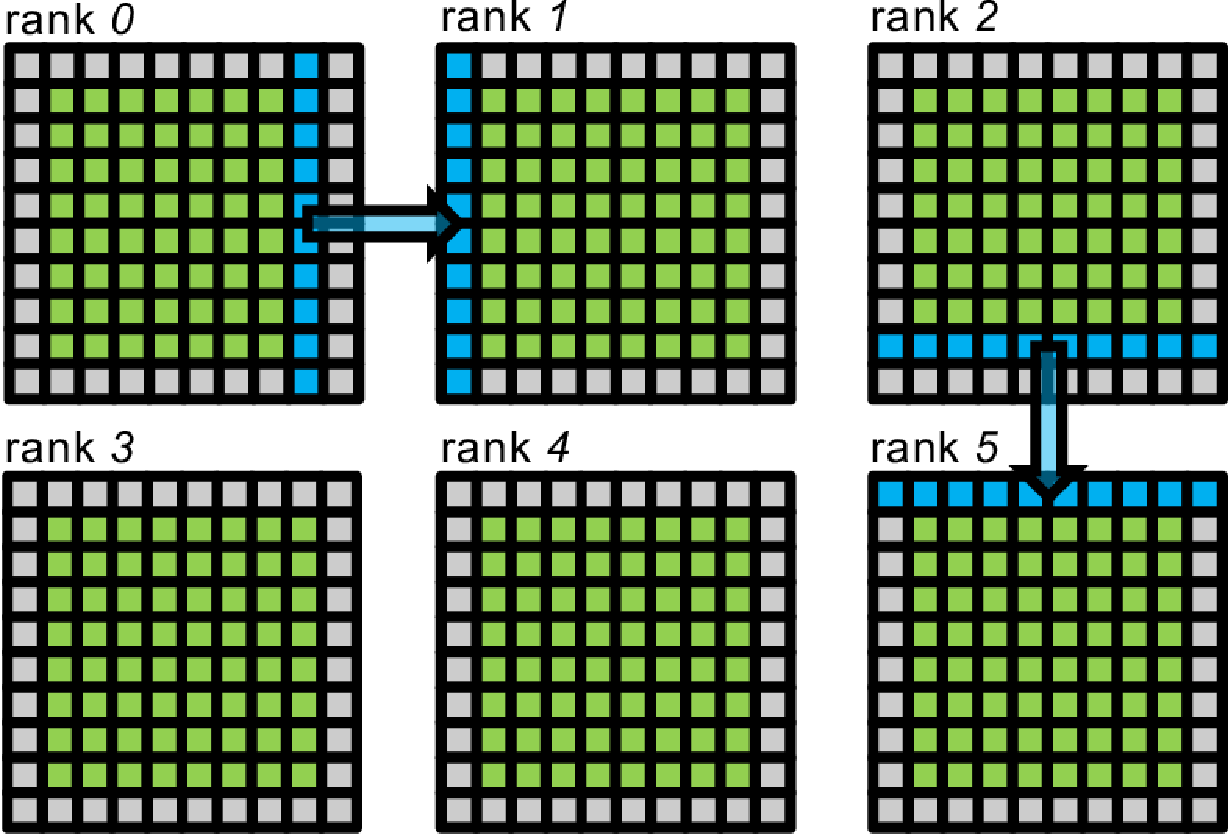
\includegraphics[width=0.48\textwidth]{imgs/mpi-conceptual.pdf}
  \caption{
    Domain decomposition and communication strategy in MPI.
    As described in the main text, we first divide each axis
    into $P_x$ and $P_y$ intervals and divide by the intervals.
    Each rank has green lattice points and this area is the active physical domain.
    Then we add additional ghost cells for buffer (gray lattice points).
    During each communication step, the outermost green active lattice
    sends the data to the adjacent outermost ghost lattice (blue arrows).
    The figure is cited from Figure~2 in ~\cite{pastewka2019hpc}.
  }
  \label{mpi-conceptual}
\end{figure}

\begin{algorithm}[b]
  \caption{The communication of
  the particle probability density function}
  \label{alg:mpi-algorithm}
  \begin{algorithmic}[1]
    \Statex{Process and lattice grids management: grid\_manager}
    \Function{communication}{}
    \State{{\bf for} dir in grid\_manager.neighbor\_directions {\bf do}}
    \Comment{Iterate over the D2Q9 index}
    \Indent
    \State{dx, dy = $\cv_i$}
    \State{sendidx = grid\_manager.step\_to\_idx(dx, dy, send=True)}
    \State{recvidx = grid\_manager.step\_to\_idx(dx, dy, send=False)}
    \State{neighbor = grid\_manager.get\_neighbor\_rank(dir)}
    \If{dx == 0} \Comment{send to top and bottom}
    \State{sendbuf = $f$[:, sendidx, ...].copy()}
    \State{grid\_manager.rank\_grid.Sendrecv(sendbuf=sendbuf, dest=neighbor,}
    \State{\hspace{56mm} recvbuf=recvbuf, source=neighbor)}
    \State{$f$[:, recvidx, ...] = recvbuf}
    \ElsIf{dy == 0} \Comment{send to left and right}
    \State{sendbuf = $f$[sendidx, ...].copy()}
    \State{grid\_manager.rank\_grid.Sendrecv(sendbuf=sendbuf, dest=neighbor,}
    \State{\hspace{56mm} recvbuf=recvbuf, source=neighbor)}
    \State{$f$[recvidx, ...] = recvbuf}
    \EndIf
    \EndIndent
    \State{{\bf return} $f$}
    \EndFunction
  \end{algorithmic}
\end{algorithm}

\section{Software quality}
All the codes follow {\tt pep8 style}~\footnote{https://www.python.org/dev/peps/pep-0008/}
and {\tt Google Python Style documentation string}~\footnote{https://google.github.io/styleguide/pyguide.html}.
In order to make the codes robust to unexpected errors,
we introduce
{\tt Flake8}~\footnote{https://flake8.pycqa.org/en/latest/}
and {\tt MyPy} static typing check~\footnote{http://mypy-lang.org/} as well.
Furthermore, all the components are tested by
{\tt unittest}\footnote{https://docs.python.org/3/library/unittest.html}
and we provide {\tt requirements.txt}
and the shell scripts for the main experiments
to reproduce the complete running conditions.
Those tools {\bf guarantee the reproducibility} of the experiments.
Furthermore, the implementations focus on abstraction and
most codes are abstracted to reduce the coding lines as much as possible.
Therefore, the codes are {\bf highly reusable} and
the implementation has only one explicit coding for
each Algorithm provided in this chapter.
Furthermore, {\tt ArgumentParser} allows users to
pass an arbitrary setting to run the experiments
and it {\bf contributes to the generality} in this code.
All the instructions are available at {\tt Github} repository
described in Chapter~1.
